
\documentclass[sigchi]{acmart}
\settopmatter{printacmref=false, printccs=true, printfolios=true}
%%
%% \BibTeX command to typeset BibTeX logo in the docs
\AtBeginDocument{%
  \providecommand\BibTeX{{%
    \normalfont B\kern-0.5em{\scshape i\kern-0.25em b}\kern-0.8em\TeX}}}

%% Rights management information.  This information is sent to you
%% when you complete the rights form.  These commands have SAMPLE
%% values in them; it is your responsibility as an author to replace
%% the commands and values with those provided to you when you
%% complete the rights form.
\setcopyright{none}
%\copyrightyear{none}
\acmYear{2021}
\acmDOI{}

%% These commands are for a PROCEEDINGS abstract or paper.
\acmConference[Technical Report]{May}{{\today}}{Cologne, Germany}
\acmBooktitle{}
\acmPrice{}
\acmISBN{}

\usepackage{subfig}

\begin{document}

\title{The impact of the avatar representation on team trust and effectiveness in a shared virtual environment.}

\author{Hannes Hinrichs}
\email{hhinrich@smail.th-koeln.de}
\affiliation{%
  \institution{TH-Köln}
  \city{Cologne}
  \country{Germany}
}

\begin{abstract}
The goal of this work is to find out if different avatar representations have an impact on the formed
trust and effectiveness of a team. The first question here is whether an inverse-kinematic humanlike
representation or an abstract non-human-like representation is more effective in generating
trust in a newly formed virtual team. The second question addresses whether the trust formed
by the different representations influences the effectiveness of the virtual team. To answer these
questions, a quantitative study was conducted in which different participants in a three-person
team performed a collaborative task in a shared virtual environment. No significant differences in
effectiveness were found between the teams. The results of the study also shows that in the threeperson
teams in the shared virtual environment, significantly more trust was built with non-humanlike
avatars, as well as that there was a significant relationship between the cognitive trust formed
and team effectiveness. This means that the simplicity of a non-human-like avatar in a newly formed
team in a shared virtual environment can be effective in creating a trusting work atmosphere.
\end{abstract}

\keywords{Virtual-Reality, Trust, Team formation, virtual Team, Avatar}

%% A "teaser" image appears between the author and affiliation
%% information and the body of the document, and typically spans the
%% page.
\begin{teaserfigure}
  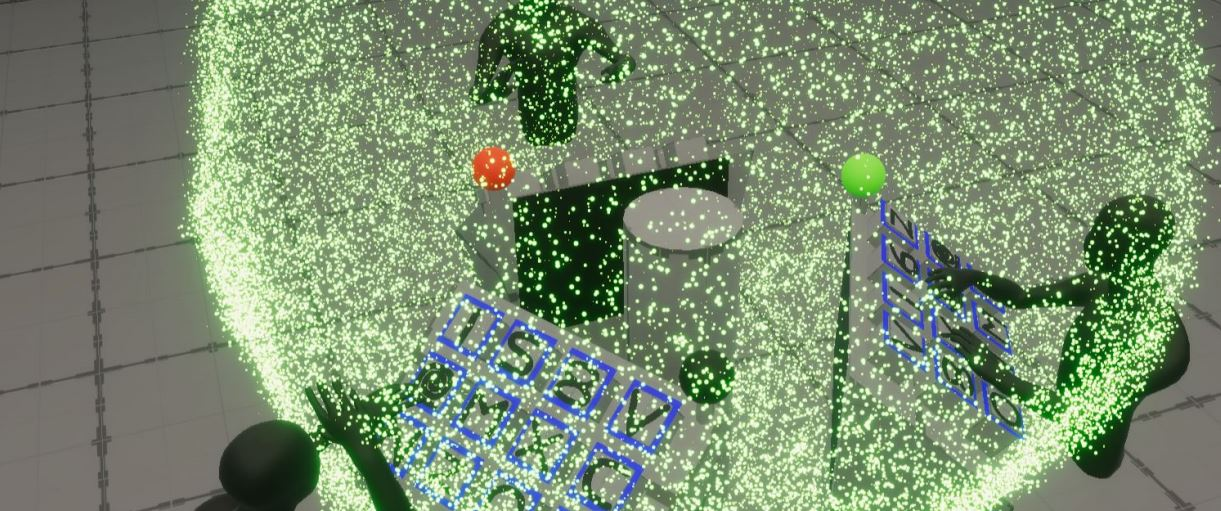
\includegraphics[width=\textwidth]{Abbildungen/RoundSuccsessful2}
  \caption{Teammembers in the Shared-Virtual-Environment}
  \Description{This figure represents the developed Shared-Virual-Environment. The green sphere appears clearly visible for all participants when a round is successfully completed.}
  \label{fig:teaser}
\end{teaserfigure}

%%
%% This command processes the author and affiliation and title
%% information and builds the first part of the formatted document.
\maketitle

\section{INTRODUCTION}
Mit voranschreitender technologischer Entwicklung rückt die digitale Kommunikation immer mehr in den Mittelpunkt. Unternehmen weltweit setzen schon seit langem darauf, räumliche und zeitliche Grenzen zu überwinden.
Neue Generationen von sozialen Netzwerksystemen werden unter der Prämisse erstellt, die Kommunikation zu entfernten Personen zu verbessern.
Einsatzfelder sind beispielsweise die \textit{Mobil- und Internettelefonie}, die\textit{ FOIP/VOIP- Telefonkonferenzen} oder die \textit{sozialen virtuellen 3D- Umgebungen}.
All diese Technologien teilen dasselbe Ziel: 
\begin{quote}
"Die Verbesserung der \textit{sozialen Präsenz}, sodass der Nutzer das Gefühl hat zu einem gewissen Grad Einblicke in die kognitiven und affektiven Zustände des anderen zu haben" \citep{biocca2002defining} \citep[S. 407–447]{biocca2001plugging}.
\end{quote}
Mitarbeiter befinden sich sehr häufig nicht am selben Ort, wobei sich viele Unternehmen trotzdem eine effektive Gestaltung ihrer Teams wünschen \citep[S. 791-792]{jarvenpaa1999communication}. \textit{Virtuelle Teams} können hierbei Abhilfe schaffen. 
Vor der Corona-Pandemie, im 2. Quartal 2020, haben 4\% aller Angestellten in Deutschland im Homeoffice gearbeitet. Dieser Anteil ist im Laufe des Jahres - Stand 01.01.2021 - auf 24\% gestiegen und es könnten theoretisch 80\% der Belegschaften von zu Hause arbeiten \citep{statistaCorona2020}. Durch diese Entwicklung mussten sich Unternehmen zwangsläufig mit der Funktionsweise von virtuellen Teams beschäftigen.
Trifft sich ein virtuelles Team in einer virtuellen Realität, können Avatare zur Repräsentation des eigenen Individuums eingesetzt werden. Durch diese wird mit anderen Teilnehmern des Shared-Virtual-Environment interagiert und kommuniziert. 
In einem räumlich getrennten Team zu arbeiten, das sich gegenseitig nicht vertraut oder nicht richtig zusammenarbeitet, hemmt dessen Performance \citep[S. 98-107]{huang1998supporting} \citep[S. 399-417]{turoff1993distributed}.
Diese Arbeit zielt darauf ab, das Konstrukt \textit{Vertrauen} in der virtuellen Welt besser zu verstehen und mit diesem umzugehen.
Es gilt herauszufinden, welche Art von Repräsentation in einem Shared-Virtual-Environment, während der Neugründung eines virtuellen Teams, mehr zwischenmenschliches Vertrauen aufbaut. Es wird ein Fokus wird auf die beiden Avatarkonditionen IK sowie NIK gelegt, um zu analysieren, ob es einen Zusammenhang zwischen dem gebildeten \textit{kognitiven Vertrauen} im Team und der \textit{Teameffektivität} bei unterschiedlichen Repräsentationsarten des Avatars während der erstmaligen Zusammenarbeit gibt.
Zudem wird sich auf das den \textit{generellen Hang zum Vertrauen} der einzelnen Personen konzentriert, um zu untersuchen, ob der \textit{generelle Hang zum Vertrauen} einen Einfluss auf die \textit{Teameffektivität} und das \textit{kognitive Vertrauen} im Hinblick auf die unterschiedlichen Konditionen besitzt. Dazu bestreitet ein Drei-Personen-Team, dessen Mitglieder sich nicht kennen, in einem Shared-Virtual-Environment eine kooperative Aufgabe.

\section{RELEATED WORD}
\subsection{TRUST}
Die meist verbreitetste Definition stammt von Meyer et al. \citep[S. 712]{mayer1995integrative}. So definieren sie Vertrauen als:
\begin{quote} "die Bereitschaft einer Person, für die Handlungen einer anderen Person anfällig zu sein, basierend auf der Erwartung, dass der Vertrauensnehmer eine bestimmte, für den Vertrauensgeber wichtige Handlung ausführen wird, unabhängig von der Möglichkeit, diese Person zu überwachen oder zu kontrollieren." \end{quote}

Jede zwischenmenschliche Beziehung beginnt mit einer frühen Phase der Vertrauensbildung. Diese frühe Phase kann von Unsicherheiten und Zweifel geprägt sein. Das gegenseitige Vertrauen, das man sich anschließend schenkt, muss anfänglich erst einmal ausgelotet werden \citep[S. 166-168]{meyerson1996swift}.
Während der frühen Phase der Vertrauensbildung entscheidet sich, ob eine Beziehung aufrechterhalten wird oder nicht. Unterbewusst bildet sich ein Gefühl von Zuversicht und Sicherheit oder ein Gefühl von Spannung, Zweifel und Skepsis dem Interaktionspartner gegenüber. 
Dabei ist es egal, ob sich dafür entschieden wird, jemandem zu vertrauen, oder nicht. Auf jeden Fall beeinflusst die Stärke des positiven oder negativen Vertrauensgefühls die Effektivität der Zusammenarbeit. Vertrauen kann es einfach oder schwierig machen, mit einer anderen Person zu arbeiten und Ziele in einer Gruppe oder einem Team zu erreichen \citep[S. 405-406]{bigley1998straining}.

Die initiale Phase der Vertrauensbildung wirkt sich auf das \textit{kognitive} und das \textit{affektive Vertrauen aus}, welche einen starken Einfluss auf das sich entwickelnde Vertrauensmodell zu einer Person haben. In dieser Phase sind diese beiden Vertrauensarten anfällig für Veränderungen \citep[S. 461-462]{baldwin1992relational}.
Meinungen und Annahmen, die sich frühzeitig bilden, prägen somit auch stark die zukünftige Meinung über die vertrauensnehmenden Personen.

Vertrauen wird nicht statisch und einseitig betrachtet. Eine Person kann nicht nur \textit{vertrauen} oder \textit{nicht vertrauen}. Vertrauen ist ein dynamisches Konstrukt, welches sich mit der Zeit verändert. Es kann in eine Bildungs-, Stabilisierungs- und Abnehmphase unterteilt werden \citep[S. 396]{rousseau1998not}.

Viele Psychologen, die sich mit dem Thema Vertrauen beschäftigen, gehen heute davon aus, dass \textit{zwischenmenschliches} Vertrauen aus einem zweidimensionalen Konstrukt besteht \citep{johnson2005cognitive}; \citep{cook1980new}. So sind Mooradian et al. der Ansicht, dass Vertrauen als \textit{Eigenschaft} oder als \textit{Zustand} gesehen wird \citep[S. 524-525]{mooradian2006trusts}.

\subsubsection{TRUST AS A TRAIT }
Wird Vertrauen als Eigenschaft betrachtet, spiegelt dies die Einstellung zum Vertrauen einer Person wider. Diese Einstellung zum Vertrauen ist langlebig und wird nicht allzu schnell auf oder abgebaut. Unabhängig von einer Situation, in der sich diese Person befindet, wird davon ausgegangen, dass diese Eigenschaft aus dem Temperament oder der Lebenserfahrung einer Person entsteht. Dieses Vertrauen ist das Grundlevel an Vertrauen, das eine Person in eine neue zwischenmenschliche Beziehung von Anfang an mitbringt \citep[S. 11]{couch1996assessment}. Es ist jedoch nicht nachgewiesen, wie \textit{generelles Vertrauen} genau gebildet wird \citep[S. 409]{stolle2002trusting}.

\textit{Generelles Vertrauen} impliziert, dass den meisten Personen vertraut werden kann, oder dass im Fall von generellem Misstrauen, Personen nicht vertraut werden kann \citep[S. 409]{stolle2002trusting}.

Der \textit{generelle Hang zum Vertrauen} ist nicht situationsabhängig, sondern stellt eine längerfristige Konstante auf Basis des Grundvertrauens einer Person dar. Grundvertrauen setzt sich dabei aus der individuellen Eigenschaft des Hangs zum Vertrauen einer einzelnen Person sowie der Grundstimmung gegenüber Personen im Allgemeinen, zusammen \citep[S. 11]{couch1996assessment}.

\subsubsection{TRUST AS A STATE}

Wird \textit{Vertrauen als Zustand} betrachtet, so kann sich dieses Vertrauen im Laufe der Zeit, z.B. durch Interaktion mit einer anderen Person, ändern \citep[S. 712]{mayer1995integrative}.
Das Konzept des \textit{Vertrauens als Zustand} lässt sich laut Lewis et al. \citep[S. 970-971]{lewis1985trust} in eine \textit{kognitive Komponente} und eine \textit{affektive Komponente} unterteilen.

\paragraph{COGNITIVE BASED TRUST}

Laut den Studie von Lewis et al. basiert unter anderem 
\begin{quote}
"auf einem kognitiven Prozess, der zwischen vertrauenswürdigen, misstrauischen und unbekannten Personen und Institutionen unterscheidet. In diesem Sinne wählen wir kognitiv aus, wem wir in welcher Hinsicht und unter welchen Umständen vertrauen, und wir stützen die Wahl auf das, was wir als "gute Gründe" ansehen, die einen Beweis für die Vertrauenswürdigkeit darstellen" \citep[S. 970]{lewis1985trust}.
\end{quote}

Somit basiert das \textbf{kognitiv aufgebaute Vertrauen} auf einer von uns definierten Logik statt auf einer emotionalen Komponente. Diese "guten Gründe" können auch leicht gebrochen werden, indem der Vertrauensvorschuss, den wir durch das kognitive Vertrauen unserem Interaktionspartner geben, gebrochen wird.
Das kognitive Vertrauen kann kurzfristig aufgebaut werden und ist leicht anfällig gegen äußerliche Einflüsse \citep[S. 970]{lewis1985trust}. 

\paragraph{AFFECTIVE BASED TRUST}

Weiterhin besitzt Vertrauen als \textit{Zustand} eine affektive Komponente:
\begin{quote}
"Diese \textbf{affektive Komponente des Vertrauens} besteht in einer emotionalen Bindung zwischen allen, die an der Beziehung beteiligt sind. Wie die affektiven Bindungen der Freundschaft und der Liebe schafft Vertrauen eine soziale Situation, in der intensive emotionale Investitionen getätigt werden können, und deshalb weckt der Verrat eines persönlichen Vertrauens ein Gefühl der emotionalen Empörung bei dem Betrogenen. Der Vertrauensbruch trifft die Grundlage der Beziehung selbst, nicht nur den spezifischen Inhalt des Verrats. Diese emotionale Komponente ist bei allen Arten von Vertrauen vorhanden, aber normalerweise ist sie bei engem zwischenmenschlichem Vertrauen am intensivsten" \citep[S. 971]{lewis1985trust}.
\end{quote}
Ein Beispiel für affektives Vertrauen ist die Liebesbeziehung zwischen zwei Personen. Das affektive Vertrauen baut sich mit der Zeit langsam auf und kann durch verschiedene Ereignisse erschüttert oder gestärkt werden. Es kann eher durch Emotionen statt durch Logik charakterisiert werden.
\textbf{Affektives Vertrauen} ergibt sich aus \textit{zwischenmenschlichen emotionalen Verbindungen und gegenseitiger Fürsorge}, während individuelles \textbf{kognitives Vertrauen} auf der \textit{Überzeugung in die Fähigkeiten oder in die Zuverlässigkeit eines anderen basiert} \citep[S. 30]{mcallister1995affect}.

\subsection{VIRTUAL TEAMS}
Ein Team wird als eine "kleine Gruppe von Menschen mit gleichartigen Fähigkeiten, welche sich in gleicher Weise für das gleiche Ziel und gleiche Arbeitsweisen einsetzen und dies verfolgen" \citep[S. 2]{zenun2007effects}, definiert.

\textit{Virtuelle Teams} teilen viele Eigenschaften herkömmlicher \textit{Teams}. Es muss jedoch unterschieden werden, wie die virtuelle Komponente des Teams definiert wird und weshalb diese Komponente ein herkömmliches Team zu einem virtuellen Team macht.

\textit{Virtuelle Teams} besitzen laut Schweizer et al. \citep[S. 270]{schweitzer2010conceptualizing} noch vier weitere Kennzeichen, um als \textit{virtuelles Team} zu gelten. Laut ihnen sind diese:
\label{AnforderungenLautSchweitzer}
\begin{itemize}
\item Zustande gekommen mithilfe von Kommunikationstechnologie. Durch technische Hilfsmittel wird kommuniziert, es werden Entscheidungen getroffen oder Informationen ausgetauscht.
\item Räumlich getrennt. \textit{Virtuelle Teams} arbeiten \textit{nicht} am selben Arbeitsplatz.
\item Grenzübergreifend. Die Teammitglieder stammen aus verschiedenen Organisationen oder Organisationseinheiten.
\item Asynchron. \textit{Virtuelle Teams} arbeiten zu unterschiedlichen Zeiten, in verschiedenen Zeitzonen oder in derselben Zeitzone in unterschiedlichen Schichten.
\end{itemize}

\textit{Virtuelle Teams} werden häufig aufgrund eines anstehenden Projektes gebildet und wieder aufgelöst, wenn das Projekt beendet ist. Somit sind \textit{virtuelle Teams}  oftmals nur von kurzer Lebensdauer. Dies impliziert auch, dass die Aufgabenverteilung in virtuellen Teams je nach Projekt oder Aufgabe immer unterschiedlich ist und keine einheitliche Hierarchie innerhalb des \textit{virtuellen Teams} zustande kommt \citep{wong2000virtual}.
Das \textit{virtuelle Team} zu gründen, stellt laut Dyer nicht die eigentliche Herausforderung dar. Die Herausforderung ergibt sich aus den unterschiedlichen Kulturen, Entfernungen und Zeitzonen, die ein \textit{virtuelles Team} mitbringt. Wenn die einzelnen Teammitglieder eines \textit{virtuellen Teams} sich gegenseitig vertrauen, kann der eigentliche Nachteil der verschiedenen Kulturen, Entfernungen und der Zeitzonen auch zum Vorteil werden. Es wird kulturelle Diversität gefordert und neue Verhaltensmuster erworben, wodurch neue, kreative Sichtweisen gefördert werden. Durch diese Faktoren ist es möglich, innovativer zu arbeiten und zu denken \citep{dyer1995team} \citep[S. 405-416]{milliken1996searching}.

Es wird davon ausgegangen, dass Virtualität als Kontinuum gesehen werden kann, bei dem jedes Team ein gewisses Maß an Virtualität besitzt. Dieses Kontinuum reicht von Face-to-Face bis zur vollständigen, nur über Kommunikationstechnologie stattfindenden Kommunikation \citep{martins2004virtual} (siehe \textit{Abbildung \ref{virtualTeamsVirtuality}}).

\begin{figure}[H]
		\begin{footnotesize}
		\centering
			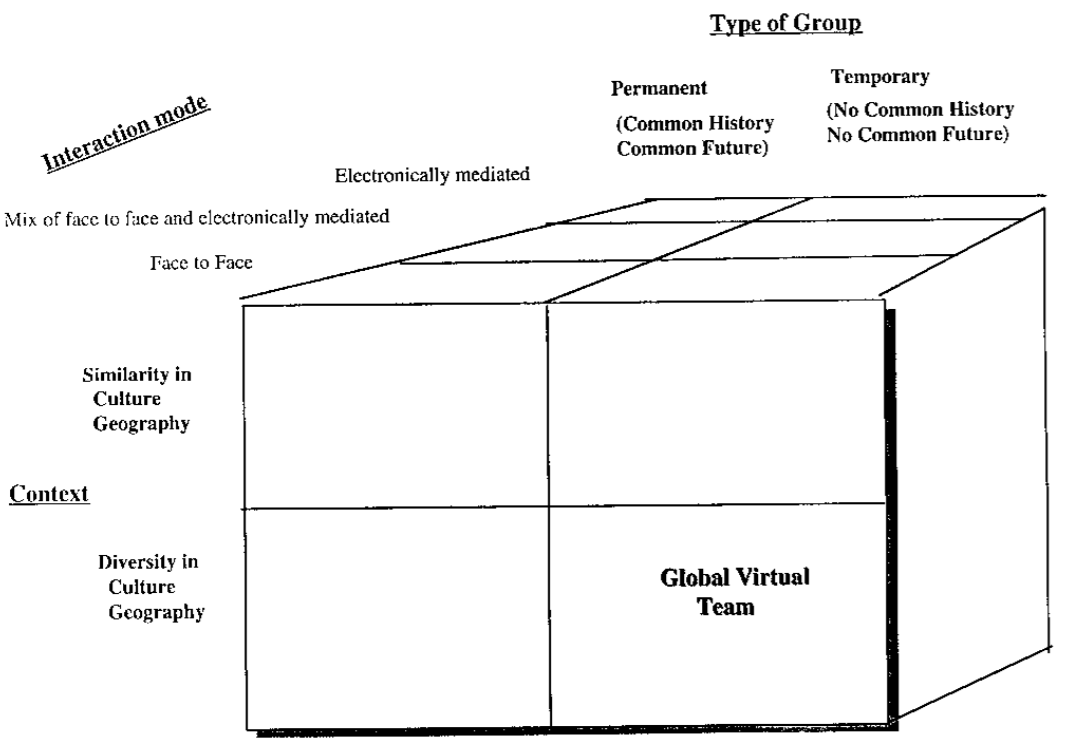
\includegraphics[width=\linewidth]{Abbildungen/GlobalVirtualTeam.PNG}	
			\caption[Virtualität eines virtuellen Teams]{Grad an Virtualität, das ein Team laut Javenpaa et al. \citep{jarvenpaa1999communication} besitzen muss, um als \textit{virtuelles Team} zu gelten.}
			\label{virtualTeamsVirtuality}
		\end{footnotesize}
	\end{figure}

Die Mitglieder eines \textit{virtuellen Teams} haben im Gegensatz zu traditionell geformten Teams weniger Möglichkeiten, sich zu sehen, zu interagieren oder Konflikte zu lösen. 
Respekt und gegenseitiges Verständnis sind die Grundbausteine, um Kreativität und Innovation innerhalb eines Teams zu fördern. Die Effektivität eines Teams ist eine direkte Konsequenz daraus \citep[S. 378]{ren2007applying}.

\paragraph{VIRTUAL TEAMS AND TEAMEFFECTIVENESS}

Wird ein Vergleich zwischen \textit{traditionell} geformten Teams und \textit{virtuellen Teams} gezogen, gehen Schweitzer et al. \citep{schweitzer2010conceptualizing} davon aus, dass traditionell geformte Teams effektiver als \textit{virtuelle Teams} sind und die \textit{Teameffektivität} abnimmt je höher der Grad an Virtualität (siehe \textit{Abbildung \ref{virtualTeamsVirtuality}}) ist.
Diese Meinung teilt auch Becker et al., denn laut ihnen leidet der Austausch des Informationsgehaltes sowie der Vertrauensbildung aufgrund steigender Virtualität und kann nicht dieselbe Effektivität wie ein Face-to-Face Team erreichen \citep{becker2002fuhrung}.
Eine andere Meinung nehmen dabei Dufner et al. ein \citep{dufner2002asynchronous}. Ein zeitlich asynchroner Informationsaustausch von \textit{virtuellen Teams} hat laut ihrer Untersuchung einen positiven Einfluss auf die \textit{Teameffektivität}, da die Teammitglieder mehr Zeit haben, um über Probleme nachzudenken, bevor Informationen ausgetauscht werden.

Bisherige Studien haben positive Zusammenhänge \citep{davis2000trusted}, keine Zusammenhänge \citep{hertel2004managing} sowie negative Zusammenhänge \citep{dirks1999effects} zwischen Vertrauen und \textit{Teameffektivität} in \textit{virtuellen Teams} festgestellt.
Trotz der sich widersprechenden Studienergebnisse wird im Allgemeinen die Meinung vertreten, dass Vertrauen einen positiven Einfluss auf die \textit{Teameffektivität} besitzt \citep{de2016trust}. 
Vertrauen in sein Team hilft dabei, eigene Unsicherheiten auszublenden, um sicherer und effektiver arbeiten zu können \citep{de2010does}. Weiterhin entsteht durch vorhandenes Vertrauen in sein Team ein größeres Interesse an den Teammitgliedern, was Synergieeffekte freischaltet und eine direktere und effektivere Interaktion ermöglicht \citep{dirks1999effects}. 

\subsection{AVATARS AND TRUST}

Es stellt sich die Frage, ob ein Avatar in einem Shared-Virtual-Environment menschenähnlich aussehen sollte. Dieser Frage gingen George et al. \citep{george2018trusting} in ihrer Forschung nach und verglichen, ob sich mehr Vertrauen zwischen einem menschenähnlichen oder einem roboterartigen Avatar aufbauen lässt.
%Dazu schufen sie ein Szenario, in dem Personen mittels eines \ac{hmd} ein Social-Dilemma-Scenario\footnote{Situationen, in denen - die rationale Verfolgung von Eigeninteressen zu einer kollektiven Katastrophe führen kann.} erlebten.
Sie fanden keinen signifikanten Unterschied in der Vertrauenswürdigkeit zwischen menschenähnlichen und roboterartigen Avataren. Jedoch wurde ein größeres Gefühl von Gemeinsamkeit festgestellt, wenn mit einem menschenähnlichen Avatar interagiert wurde.
% \citep{kerr1983motivation}.
George et al. erwähnten weiterhin in ihrer Studie, dass gute Grafik und realistisches Verhalten durch beispielsweise Mikrogestikulationen und soziale Interaktionen den Aufbau von \textit{Co-Präsenz} unterstützen \citep{george2018trusting}.

Um den Einfluss des Grades an Realismus unter Avataren zu erforschen, führten Riedl et al. \citep{riedl2014trusting} eine Studie zum Vertrauensaufbau unter Menschen im Vergleich zu Avataren mit menschenähnlichen Gesichtern durch. Sie fanden heraus, dass es Personen leichter fällt, einer realen Person, zu vertrauen als einem Avatar mit menschenähnlichem Gesicht. Es wurde der Frontalkortex - die Gehirnregion, die dafür verantwortlich ist, die Gedanken und Gefühle des Gegenübers zu erahnen - bei Interaktionen mit Menschen mehr angeregt als bei Interaktionen mit Avataren mit menschenähnlichen Gesichtern.
Vertrauen zwischen Menschen wird jedoch in der gleichen Geschwindigkeit aufgebaut wie zwischen Menschen und Avataren.

Somit lässt sich feststellen, dass ein höherer Grad an Realismus den Vertrauensaufbau fördert, jedoch kein signifikanter Unterschied in der Geschwindigkeit  des Vertrauensaufbaus zwischen einem menschenähnlichen sowie roboterähnlichen Avatar besteht. Diese Vermutung bestätigten auch Bente et al. \citep[S. 54-59]{bente2004social}, indem sie eine Studie zur \textit{sozialen Präsenz} von Avataren in einem \textit{Shared-Virtual-Environment} durchführten. Der Aufbau des \textit{Shared-Virtual-Environment} ähnelte einer Videokonferenz. Es waren keine \textit{Head-Mounted-Display}s vorhanden und die Teilnehmer haben sich während des Experiments nicht gesehen. In der Studie wurden die Kommunikationsarten, Face-to-Face, Chat und auf Avataren basierende Kommunikationsmedien untereinander verglichen, um Unterschiede in der \textit{Sozialen-Präsenz} sowie dem zwischenmenschlichen Vertrauen zu untersuchen.
Es wurde festgestellt, dass wenig \textit{kognitives Vertrauen} während der Nutzung des \textit{Shared-Virtual-Environment} zu Avataren aufgebaut werden konnte, während Face-to-Face, Telefon- und Chatkommunikationen besser abschnitten. Weiterhin wurde weniger \textit{affektives Vertrauen} im \textit{Shared-Virtual-Environment} als bei der Nutzung eines Telefons oder während der Face-to-Face Kommunikation aufgebaut.
Bente et al. \citep[S. 54-59]{bente2004social} gehen davon aus, dass dies mit der Neuheit der Technologie zusammenhängt.

\section{METHODS}

Um die beiden unabhängigen Variablen IK und NIK innerhalb der Versuchsumgebung zu untersuchen, wird das \textit{A/B-Testing} in Kombination mit einem induktiven quantitativen Forschungsdesign gewählt.
Gruppe A bekommt dabei die Kondition IK zugeteilt, während Gruppe B die Kondition NIK zugeteilt wird. Diese Gruppeneinteilung der Probanden erfolgt nach dem Zufallsprinzip. 

Die Analysen dieser Studie werden auf unterschiedlichen Ebenen durchgeführt.
Da die Teilnehmer als Team arbeiten und unterschiedliche Teams unterschiedliche Konditionen aufweisen, sind einige Zusammenhänge auf \textit{Individualebene}, einige auf \textit{Konditionsebene} und einige auf \textit{Teamebene} zu betrachten.

Die \textbf{Individualebene} sagt etwas über eine einzelne Person aus. Dadurch können alle Teilnehmer individuell betrachtet werden. Die Betrachtung ist dabei unabhängig vom Team oder den verschiedenen Avatar-Konditionen. 

Die \textbf{Konditionsebene} unterscheidet zwischen den Konditionen IK und NIK. Die Konditionsebene ordnet den einzelnen Teilnehmern die Kondition zu, die diese im Shared-Virtual-Environment als \textit{andere} Avatare wahrnehmen. 

Die Konditionsebene kann in einzelne Teams von jeweils 3 Personen aufgeteilt werden. Diese Aufteilung wird als \textbf{Teamebene} bezeichnet und betrachtet das gesamte Team als Einheit. Jedes Teammitglied besitzt dieselbe Kondition. Wird das Team auf Teamebene betrachtet, ist es möglich Aussagen über das Team zu treffen. 
Die \textit{Abbildung \ref{DifferentLevels}} zeigt die Hierarchie der verschiedenen Ebenen.

\begin{figure}[H]
		\begin{footnotesize}
		\centering
			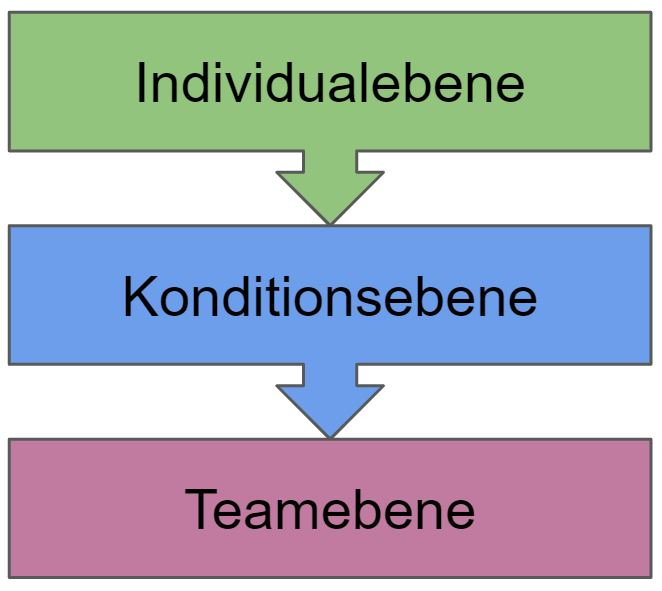
\includegraphics[width=0.5\linewidth]{Abbildungen/DifferentLevels.JPG}	
			\caption[Die Hierarchieebenen]{Die Hierarchie der Individualebene, Konditionsebene und Teamebene.}
			\label{DifferentLevels}
		\end{footnotesize}
	\end{figure}

\paragraph{Generelles Vertrauen}
Es wird der Zusammenhang zwischen dem \textit{generellen Vertrauen} und dem \textit{kognitiven Vertrauen} auf \textit{Konditionsebene} analysiert.
Es wird auf \textit{Teamebene} analysiert, ob ein Zusammenhang zwischen dem \textit{generellen Vertrauen} und der \textit{Teameffektivität} besteht.

\paragraph{Kognitives Vertrauen}
Es wird der Zusammenhang zwischen dem \textit{gebildeten kognitiven Vertrauen} und der \textit{Teameffektivität} auf \textit{Teamebene} analysiert.

\paragraph{Avatar-Darstellung}
Es wird der \textit{Unterschied} zwischen dem \textit{gebildeten kognitiven Vertrauen} bei unterschiedlichen Avatar-Konditionen auf \textit{Konditionsebene} analysiert.
Es wird der \textit{Unterschied} \textit{der Teameffektivität} bei unterschiedlichen Avatar-Konditionen auf \textit{Teamebene} analysiert.

Anhand des im Folgenden grafisch dargestellten Frameworks (siehe \textit{Abbildung \ref{Versuchshypothesen}}) wurden Hypothesen entwickelt, die im nächsten Kapitel genauer definiert und erklärt werden.

\begin{figure}[H]
		\begin{footnotesize}
			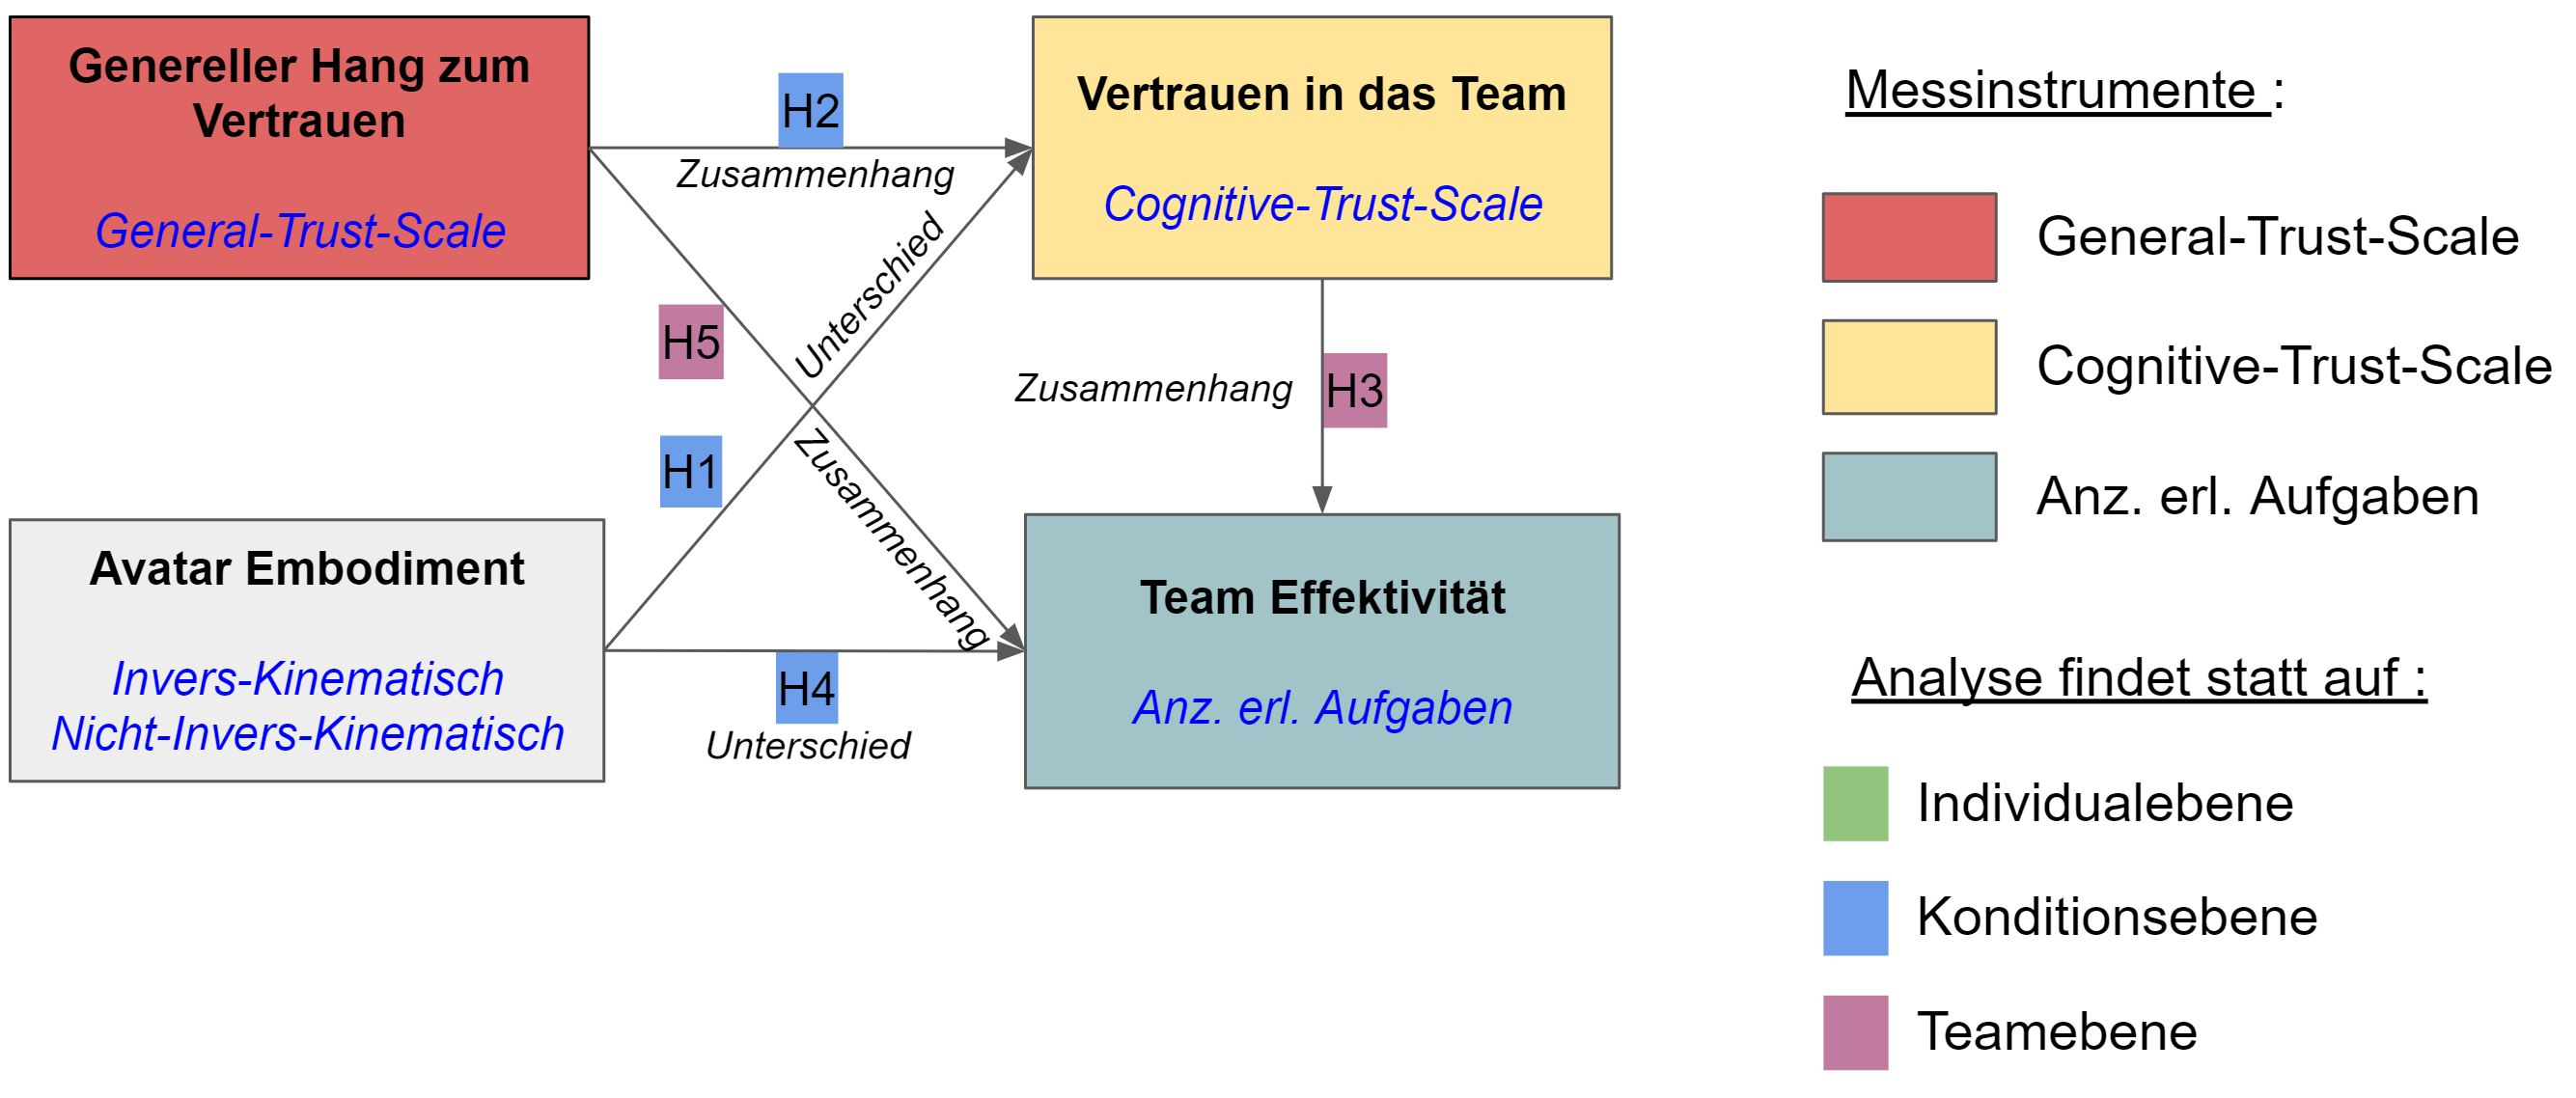
\includegraphics[width=\linewidth]{Abbildungen/Versuchshypothesen_02.JPG}		
			\caption[Das Framework der Versuchshypothesen]{Dieses Framework verdeutlicht, wie die Hypothesen zusammenhängen.}
			\label{Versuchshypothesen}
		\end{footnotesize}
	\end{figure}	

Es wurden folgende Hypothesen aufgestellt :

\textbf{H1$_{1}$}: Die Mittelwerte der erzielten \textit{kognitiven Vertrauenswerte} unterscheiden sich bei den Konditionen IK und NIK signifikant voneinander.

\textbf{H2$_{1}$}: Je höher der erzielte \textit{generelle Vertrauenswert} einer Person ist, desto höher ist der erzielte \textit{kognitive Vertrauenswert} einer Person.

\textbf{H3$_{1}$}: Der Zusammenhang zwischen dem \textit{kognitiven Vertrauenswert von Teams} und der \textit{Teameffektivität von Teams} mit der Kondition IK ist stärker als der von Teams mit der Kondition NIK.

\textbf{H4$_{1}$}: Die Mittelwerte der \textit{Teameffektivität} unterscheiden sich bei den Konditionen IK und NIK signifikant voneinander.

\textbf{H5$_{1}$}: Der Zusammenhang zwischen dem \textit{generellen Vertrauenswert eines Teams} und der \textit{Teameffektivität eines Teams} mit der Kondition IK ist stärker als der von Teams mit der Kondition NIK.

\begin{itemize}
\item \textbf{Generelles Vertrauen} Das generelle Vertrauen bezieht sich in dieser Studie darauf, wie sehr die Teilnehmer dazu neigen, anderen Personen einen Vertrauensvorschuss zu gewähren. \citep[S. 30]{mcallister1995affect}.
\item \textbf{Kognitives Vertrauen} Das \textit{kognitive Vertrauen} bezieht sich auf die \textit{Überzeugung in die Fähigkeiten oder in die Zuverlässigkeit eines anderen} \citep[S. 30]{mcallister1995affect}.
\item \textbf{Teameffektivität} Die \textit{Teameffektivität} wird anhand der Anzahl der abgeschlossenen Runden im Team gemessen.
\end{itemize}

\subsection{MEASURING METHODS}
Der General-Trust-Scale ($\alpha =,91$) \citep{couch1996assessment} wurde eingesetzt, um den generellen Vertrauenswert der einzelnen Teilnehmer zu messen. 

Der Cognitive-Trust-Scale ($\alpha =,91$) Fragebogen ist ein Auszug des von McAllister et al. \citep[S. 37]{mcallister1995affect} entwickelten Fragebogens. Er überprüft, wie viel \textit{kognitives Vertrauen} die Teilnehmer während des Versuchs aufbauen.

Gonzales-Rom et al. \citep[S. 1049]{gonzalez2014climate} entwickelten 2004 einen Fragebogen, um die \textit{Qualität von Teamkommunikation} ($\alpha =,76$) zu messen.

Gibson et al. \citep[S. 469]{gibson2003team} entwickelten 2003 einen Fragebogen, der die \textit{wahrgenommene Teameffektivität} ($\alpha =,62-,88$) misst. In dieser Studie wurde ein Auszug des Fragebogens verwendet. Er misst das \textit{subjektive Ausmaß der wahrgenommenen Teameffektivität}.

Der NASA-TLX ($\alpha =,84$) erfragt die allgemeine Belastung der Probanden, die sie während des Experiments empfunden haben. 

Der IPQ ($\alpha =,85$) dient zur \textit{Messung des Präsenz-Gefühls} in einer virtuellen Umgebung. Er misst, inwieweit sich der Nutzer in der virtuellen Umgebung anwesend fühlt, inwieweit der Nutzer seine Aufmerksamkeit der virtuellen Umgebung schenkt und wie real die virtuelle Umgebung dem Nutzer erschien. 

Mithilfe des \textit{Co-Präsenz-Fragebogens} können die \textit{selbst gemeldete Co-Präsenz} ($\alpha =,78$), die \textit{wahrgenommene Präsenz des anderen} ($\alpha =,90$), die \textit{Telepräsenz} ($\alpha =,88$) sowie die \textit{soziale Präsenz} ($\alpha =,82$) ermittelt werden.
\subsection{PARTICIPANTS}

Die Teilnehmer werden über zwei Wege akquiriert. Zum einen werden im Bekanntenkreis Personen angesprochen, denen die notwendige Hardware zur Verfügung gestellt wird. Zum anderen werden in verschiedenen Foren (z.B. VRForum.de, Computerbase.de, Hardwareluxx.de, etc.) in Form eines extra dafür angelegten Threads Teilnehmer gesucht, die an der Studie teilnehmen wollen. Weiterhin werden Teilnehmer mithilfe verschiedener sozialer Netzwerke mit einem Bezug zu VR sowie zufälliger WhatsApp-Chatgruppen mit 50 oder mehr Mitgliedern akquiriert. Da der gesamte Versuch, die Fragebögen sowie das Erklärvideo auf deutscher Sprache erstellt wurde, findet die Teilnehmerfindung nur im deutschsprachigen Raum statt.

Um an dem Experiment teilnehmen zu können, benötigen die Teilnehmer ein in vollem Umfang funktionierendes SteamVR, Windows-Mixed-Reality oder ein Oculus Rift/Rift-S Head-Mounted-Display mit kompatiblen Controllern sowie einen leistungsstarken VR-fähigen PC. Der Spectator, der das Experiment von außerhalb steuert und verwaltet, nutzt einen PC, auf dem die Anwendung ohne Head-Mounted-Display ausführbar ist.

\subsection{PROCEDURE}
Zunächst wird jedem Team entweder die Kondition IK oder NIK zugeordnet. Es gab fünf Teams mit der Kondition IK sowie fünf Teams mit der Kondition NIK.
Es werden jeweils drei Personen in einem Zeitslot untergebracht, um ein Team zu bilden. Insgesamt nehmen somit drei Personen an einem Versuch zur selben Zeit mit derselben Kondition teil. Die Teilnehmer werden sich untereinander \textit{nicht} Face-to-Face vorgestellt und sehen sich während des gesamten Experiments nur als Repräsentation eines Avatars im Shared-Virtual-Environment . 
Ein Zeitslot wird auf 25 Minuten festgelegt und teilt sich auf in
		\begin{itemize}
			\item 5 Minuten Pre-Questionnaire,
			\item 5 Minuten Videoerklärung,
			\item 10 Minuten Versuchsdurchführung,
			\item 15 Minuten Post-Questionnaire.
		\end{itemize}
Jeder Teilnehmer bekommt zu Beginn seines Zeitslots einen Pre-Questionnaire ausgehändigt, den er selbstständig ausfüllt. Alle Teilnehmer schauen sich anschließend ein Erklärvideo über das Experiment an, in dem alle relevanten Mechaniken und Funktionsweisen sowie der grobe Spielablauf erklärt werden. Durch das Erklärvideo wird sichergestellt, dass alle teilnehmende Person denselben Informationsgehalt über die Art und Weise des Ablaufs des Experiments besitzen. Alle Mitglieder eines Teams starten dadurch mit einem einheitlichen Wissensstand. Nachdem alle Personen die Videoerklärung angeschaut haben, beginnt das Experiment. Dazu starten die jeweiligen Teilnehmer die Anwendung. Es wird sich automatisch mit dem Online-Server des Shared-Virtual-Environment verbunden. Die Teilnehmer haben nun 10 Minuten Zeit, möglichst viele Runden im Team zu absolvieren. Am Ende der Versuchsdurchführung wird ein Post-Questionnaire ausgeteilt, den die Teilnehmer ausfüllen müssen. Die maximale Versuchsdauer nach Start der Anwendung beträgt exakt 10 Minuten (600 Sekunden) und es können maximal 15 Runden absolviert werden. Die Runden werden dabei inkrementell schwieriger, da in jeder dritten Runde jeweils ein Symbol in den Pool der zu erratenden Symbole hinzukommt.
 \textit{Abbildung \ref{RoundDifficulty}} zeigt die steigenden Schwierigkeitswerte, anhand derer in diesem Experiment die \textit{Teameffektivität} gemessen wurde.

\begin{figure}[H]
		\begin{footnotesize}
		\centering
			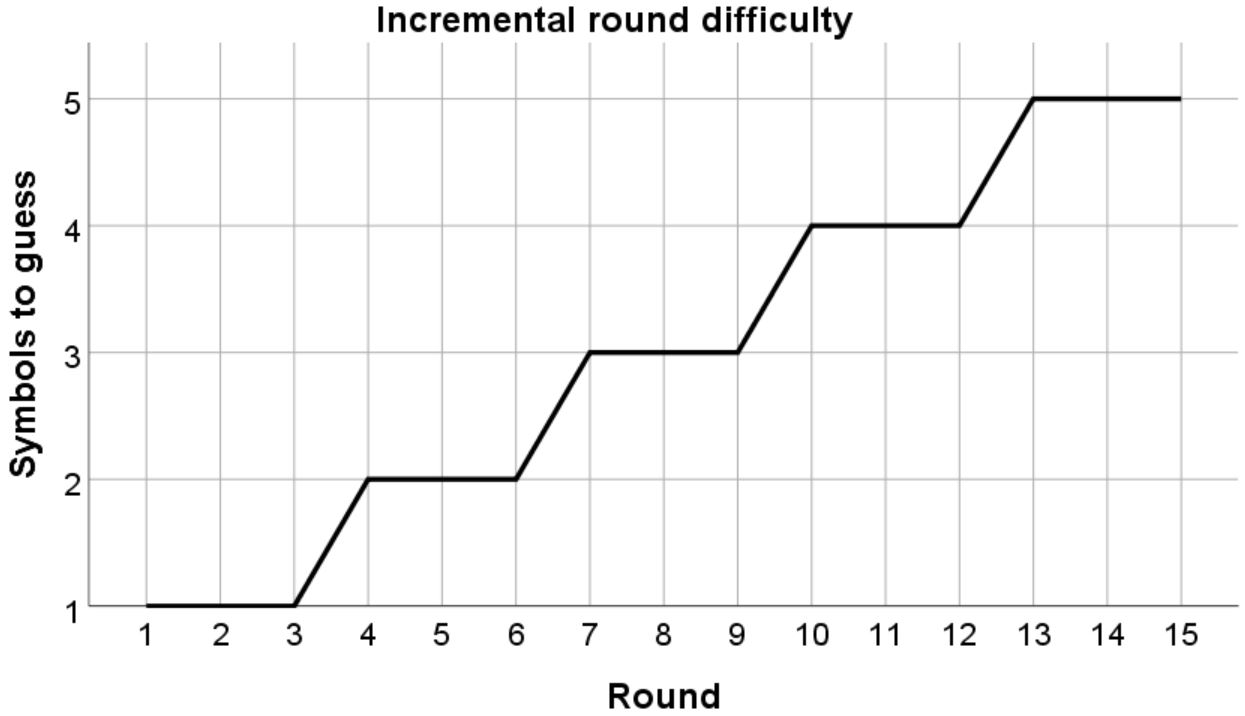
\includegraphics[width=\linewidth]{Abbildungen/RoundDifficulty.JPG}	
			\caption[Der Schwierigkeitsgrad der Runden]{Die steigende Schwierigkeit der zu erratenden Symbole der einzelnen Runden. In Runde 1-3 muss ein Symbol erraten werden, in Runde 3-6 zwei Symbole usw.}
			\label{RoundDifficulty}
		\end{footnotesize}
	\end{figure}

Zu Beginn jeder neuen Runde können die Spieler die Zuteilung der Farben sehen und dadurch den Startspieler identifizieren. Dieser ist schwarz markiert und hat die Aufgabe, seinen Mitspielern die für ihn farblich gekennzeichneten Symbole zu erklären. Seine Mitspieler müssen die ihnen zugeteilten Symbole identifizieren und an ihrem Podest einloggen. Das Ziel ist, so viele Symbole wie möglich individuell korrekt zu erkennen, um dadurch gemeinsam in höhere Runden aufzusteigen.

Die Symbole auf dem Podest des schwarz markierten Spielers sind entweder durch die Farbe Grün, Rot oder Grün-Rot gekennzeichnet. Auf den Podesten der Mitspieler befinden sich ebenfalls Symbole, welche jedoch zufällig angeordnet sind und keine farblichen Markierungen haben. Der schwarz markierte Spieler versucht nun, mittels Hand- und Armbewegung, den rot und grün markierten Mitspielern die Symbole, die in der jeweiligen Spielerfarbe vor ihm markiert sind, zu erklären. Meint der gerade angesprochene Mitspieler ein Symbol erkannt zu haben, loggt dieser das Symbol durch das Herunterdrücken des passenden Knopfes an seinem Podest ein. Hat sich ein Spieler während des Einloggens der Symbole verklickt oder möchte seine Angabe ändern, muss das Symbol durch erneutes Herunterdrücken ausgeloggt werden. Anschließend kann es erneut eingeloggt werden. 

Werden alle gekennzeichneten Symbole vom roten und grünen Spieler erkannt und eingeloggt, erscheint eine leuchtend grüne Kugel, die das Ende einer Runde anzeigt. Erscheint diese grüne Kugel nicht, ist noch ein Symbol falsch eingeloggt und der schwarz markierte Spieler muss noch einmal versuchen, die korrekten Symbole den jeweiligen Mitspielern aufzuzeigen. 
In der nächsten Runde wird ein anderer Spieler eindeutig mit Schwarz, Rot oder Grün markiert.
In der folgenden Runde erhält jeder Spieler wieder eine andere der drei Farben. Mit steigender Anzahl an erfolgreich bestandenen Runden müssen immer mehr Symbole richtig erkannt werden.
\textit{Abbildung \ref{AvatareImEinsatz}} zeigt beide Avatar-Konditionen IK (a) und NIK (b) während der Versuchsdurchführung im Spectatorview.
	
\begin{figure}[h]
  \centering
  \subfloat[][]{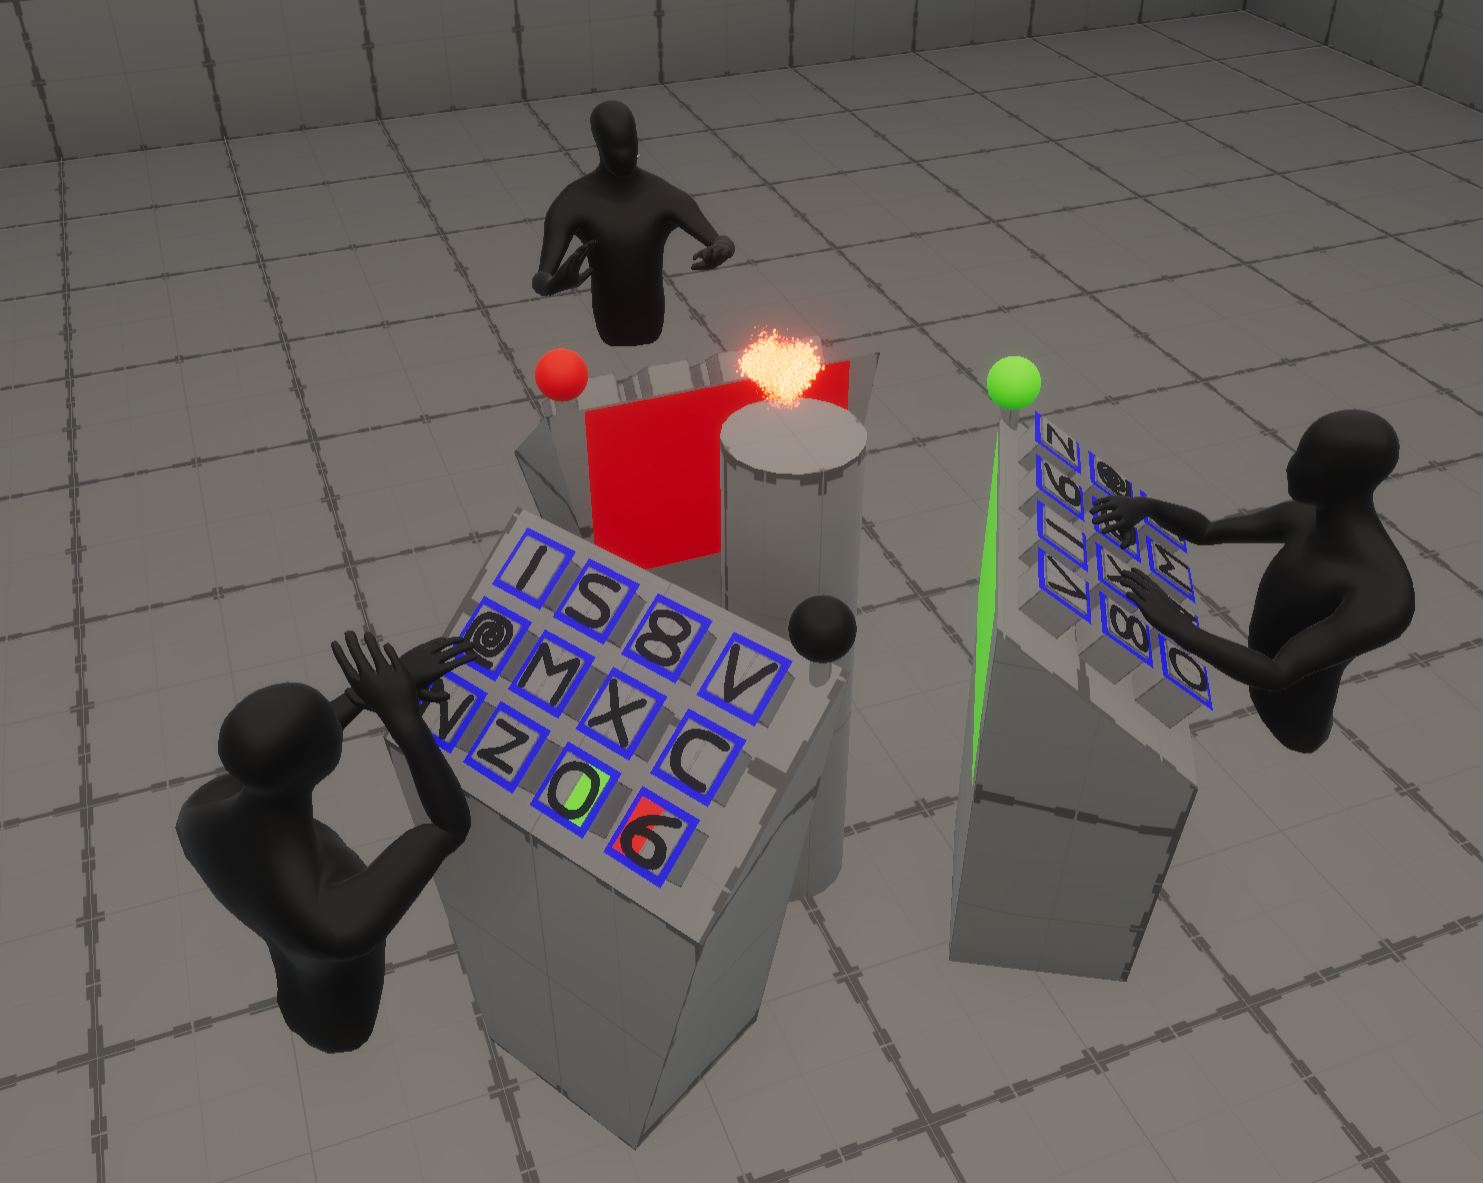
\includegraphics[width=0.45\linewidth]{Abbildungen/Podeste_IK_Avatars.jpg}}
  \qquad
  \subfloat[][]{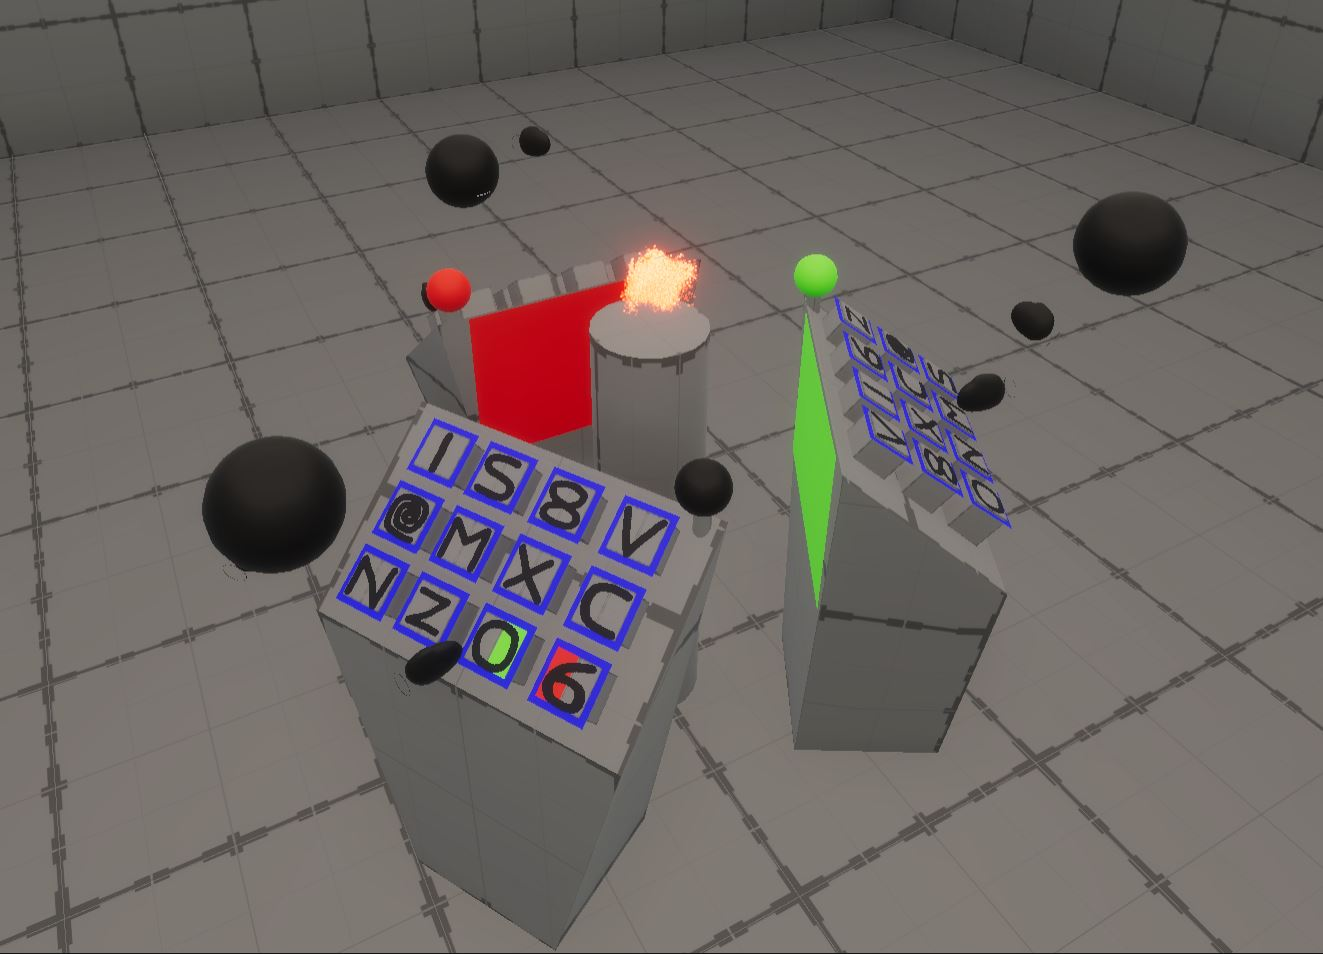
\includegraphics[width=0.45\linewidth]{Abbildungen/Podeste_Non_IK_Avatars.jpg}}
  \caption[Die Avatare und der Spectatorview]{Avatar-Konditionen IK (a) und NIK (b) während der Versuchsdurchführung im Spectatorview.}
  \label{AvatareImEinsatz}
\end{figure}

\subsection{IMPLEMENTATION}

Um den Versuch durchzuführen, wurde ein Shared-Virtual-Environment entwickelt, in dem sich die drei Teammitglieder gegenseitig als Avatare sehen und miteinander interagieren können. Das Shared-Virtual-Environment ist mit Unity 2019.4.3f1 und der HD-Render-Pipeline entwickelt worden. Um die Echtzeitkommunikation zwischen den einzelnen Clients zu gewährleisten, wurde das Multiplayer-Framework \textit{Normcore v2.0}\footnote{www.Normcore.io} genutzt.

\subsubsection{AVATAR}
	\paragraph{IK-Avatar}
Der Avatar hat keine Augen, Mund, Haare oder Beine. Lediglich der Oberkörper, der Kopf sowie die Arme sind zu erkennen. Dieser Avatar besitzt somit keine Beine und schwebt mit dem Torso über dem Boden.
Die Handbewegungen, die Unterarmbewegungen, die Oberarmbewegungen sowie die Kopf- und Torsorotation des Avatar IK werden invers-kinematisch dargestellt. Die Positions- und Rotationsdaten für den Kopf und den Oberkörper werden über das Head-Mounted-Display gewonnen. Die Positions- und Rotationsdaten der Arme werden über die beiden Controller gewonnen.

		\paragraph{Non-IK-Avatar}
Der NIK-Avatar besteht aus einer Kugel mit Mund sowie einer Repräsentation der linken und der rechten Hand. Durch den fehlenden Oberkörper und die fehlenden Beine, schwebt der Avatar über dem Boden. Der Kopf ist frei beweglich und unabhängig von den Händen. Der Mund des Avatars bewegt sich nicht, sondern dient am Kopf als Orientierungspunkt. Dadurch kann ausgemacht werden, in welche Richtung der Kopf des Avatars gedreht ist. Die Positions- und Rotationsdaten für den Kopf werden über das Head-Mounted-Display gewonnen. Die Positions- und Rotationsdaten für die Hände werden über die beiden Controller gewonnen.\\
\textit{Abbildung \ref{AvatareImEinsatz}} zeigt beide Avatar-Konditionen IK (a) und NIK (b) während der Versuchsdurchführung im Spectatorview.

	\begin{figure}[H]
		\begin{footnotesize}
		\centering
			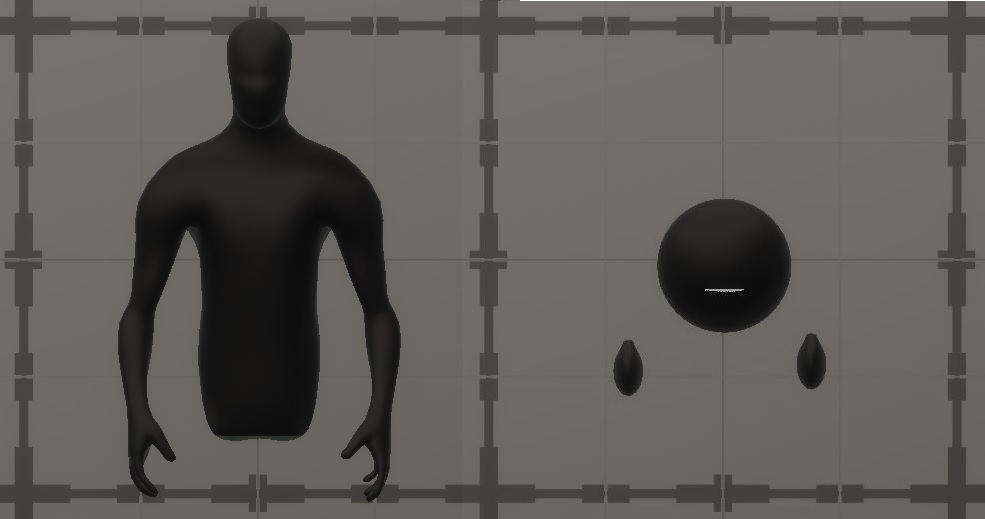
\includegraphics[width=\linewidth]{Abbildungen/Avatars.JPG}	
			\caption[Die verwendeten Avatare]{Die verwendeten Avatare : Links: IK-Avatar und rechts: Non-IK-Avatar.}
			\label{AvatareAussehen}
		\end{footnotesize}
	\end{figure}

\subsubsection{THE ENVIRONMENT}


\paragraph{USER TEST}

\paragraph{THE TEST ENVIRONMENT}

\section{STATISTICAL RESULTS}

\section{RESULTS}

\subsection{DISCUSSION}

\subsection{LIMITATIONS}

\section{CONCLUSION}

The primary parameter given to the ``\verb|acmart|'' document class is
the {\itshape template style} which corresponds to the kind of publication
or SIG publishing the work. This parameter is enclosed in square
brackets and is a part of the {\verb|documentclass|} command:
\begin{verbatim}
  \documentclass[STYLE]{acmart}
\end{verbatim}

Journals use one of three template styles. All but three ACM journals
use the {\verb|acmsmall|} template style:
\begin{itemize}
\item {\verb|acmsmall|}: The default journal template style.
\item {\verb|acmlarge|}: Used by JOCCH and TAP.
\item {\verb|acmtog|}: Used by TOG.
\end{itemize}

The majority of conference proceedings documentation will use the {\verb|acmconf|} template style.
\begin{itemize}
\item {\verb|acmconf|}: The default proceedings template style.
\item{\verb|sigchi|}: Used for SIGCHI conference articles.
\item{\verb|sigchi-a|}: Used for SIGCHI ``Extended Abstract'' articles.
\item{\verb|sigplan|}: Used for SIGPLAN conference articles.
\end{itemize}

\subsection{Template Parameters}

In addition to specifying the {\itshape template style} to be used in
formatting your work, there are a number of {\itshape template parameters}
which modify some part of the applied template style. A complete list
of these parameters can be found in the {\itshape \LaTeX\ User's Guide.}

Frequently-used parameters, or combinations of parameters, include:
\begin{itemize}
\item {\verb|anonymous,review|}: Suitable for a ``double-blind''
  conference submission. Anonymizes the work and includes line
  numbers. Use with the \verb|\acmSubmissionID| command to print the
  submission's unique ID on each page of the work.
\item{\verb|authorversion|}: Produces a version of the work suitable
  for posting by the author.
\item{\verb|screen|}: Produces colored hyperlinks.
\end{itemize}

This document uses the following string as the first command in the
source file:
\begin{verbatim}
\documentclass[sigconf]{acmart}
\end{verbatim}

\section{Modifications}

Modifying the template --- including but not limited to: adjusting
margins, typeface sizes, line spacing, paragraph and list definitions,
and the use of the \verb|\vspace| command to manually adjust the
vertical spacing between elements of your work --- is not allowed.

{\bfseries Your document will be returned to you for revision if
  modifications are discovered.}

\section{Typefaces}

The ``\verb|acmart|'' document class requires the use of the
``Libertine'' typeface family. Your \TeX\ installation should include
this set of packages. Please do not substitute other typefaces. The
``\verb|lmodern|'' and ``\verb|ltimes|'' packages should not be used,
as they will override the built-in typeface families.

\section{Title Information}

The title of your work should use capital letters appropriately -
\url{https://capitalizemytitle.com/} has useful rules for
capitalization. Use the {\verb|title|} command to define the title of
your work. If your work has a subtitle, define it with the
{\verb|subtitle|} command.  Do not insert line breaks in your title.

If your title is lengthy, you must define a short version to be used
in the page headers, to prevent overlapping text. The \verb|title|
command has a ``short title'' parameter:
\begin{verbatim}
  \title[short title]{full title}
\end{verbatim}

\section{Authors and Affiliations}

Each author must be defined separately for accurate metadata
identification. Multiple authors may share one affiliation. Authors'
names should not be abbreviated; use full first names wherever
possible. Include authors' e-mail addresses whenever possible.

Grouping authors' names or e-mail addresses, or providing an ``e-mail
alias,'' as shown below, is not acceptable:
\begin{verbatim}
  \author{Brooke Aster, David Mehldau}
  \email{dave,judy,steve@university.edu}
  \email{firstname.lastname@phillips.org}
\end{verbatim}

The \verb|authornote| and \verb|authornotemark| commands allow a note
to apply to multiple authors --- for example, if the first two authors
of an article contributed equally to the work.

If your author list is lengthy, you must define a shortened version of
the list of authors to be used in the page headers, to prevent
overlapping text. The following command should be placed just after
the last \verb|\author{}| definition:
\begin{verbatim}
  \renewcommand{\shortauthors}{McCartney, et al.}
\end{verbatim}
Omitting this command will force the use of a concatenated list of all
of the authors' names, which may result in overlapping text in the
page headers.

The article template's documentation, available at
\url{https://www.acm.org/publications/proceedings-template}, has a
complete explanation of these commands and tips for their effective
use.

Note that authors' addresses are mandatory for journal articles.

\section{Rights Information}

Authors of any work published by ACM will need to complete a rights
form. Depending on the kind of work, and the rights management choice
made by the author, this may be copyright transfer, permission,
license, or an OA (open access) agreement.

Regardless of the rights management choice, the author will receive a
copy of the completed rights form once it has been submitted. This
form contains \LaTeX\ commands that must be copied into the source
document. When the document source is compiled, these commands and
their parameters add formatted text to several areas of the final
document:
\begin{itemize}
\item the ``ACM Reference Format'' text on the first page.
\item the ``rights management'' text on the first page.
\item the conference information in the page header(s).
\end{itemize}

Rights information is unique to the work; if you are preparing several
works for an event, make sure to use the correct set of commands with
each of the works.

The ACM Reference Format text is required for all articles over one
page in length, and is optional for one-page articles (abstracts).

\section{CCS Concepts and User-Defined Keywords}

Two elements of the ``acmart'' document class provide powerful
taxonomic tools for you to help readers find your work in an online
search.

The ACM Computing Classification System ---
\url{https://www.acm.org/publications/class-2012} --- is a set of
classifiers and concepts that describe the computing
discipline. Authors can select entries from this classification
system, via \url{https://dl.acm.org/ccs/ccs.cfm}, and generate the
commands to be included in the \LaTeX\ source.

User-defined keywords are a comma-separated list of words and phrases
of the authors' choosing, providing a more flexible way of describing
the research being presented.

CCS concepts and user-defined keywords are required for for all
articles over two pages in length, and are optional for one- and
two-page articles (or abstracts).

\section{Sectioning Commands}

Your work should use standard \LaTeX\ sectioning commands:
\verb|section|, \verb|subsection|, \verb|subsubsection|, and
\verb|paragraph|. They should be numbered; do not remove the numbering
from the commands.

Simulating a sectioning command by setting the first word or words of
a paragraph in boldface or italicized text is {\bfseries not allowed.}

\section{Tables}

The ``\verb|acmart|'' document class includes the ``\verb|booktabs|''
package --- \url{https://ctan.org/pkg/booktabs} --- for preparing
high-quality tables.

Table captions are placed {\itshape above} the table.

Because tables cannot be split across pages, the best placement for
them is typically the top of the page nearest their initial cite.  To
ensure this proper ``floating'' placement of tables, use the
environment \textbf{table} to enclose the table's contents and the
table caption.  The contents of the table itself must go in the
\textbf{tabular} environment, to be aligned properly in rows and
columns, with the desired horizontal and vertical rules.  Again,
detailed instructions on \textbf{tabular} material are found in the
\textit{\LaTeX\ User's Guide}.

Immediately following this sentence is the point at which
Table~\ref{tab:freq} is included in the input file; compare the
placement of the table here with the table in the printed output of
this document.

\begin{table}
  \caption{Frequency of Special Characters}
  \label{tab:freq}
  \begin{tabular}{ccl}
    \toprule
    Non-English or Math&Frequency&Comments\\
    \midrule
    \O & 1 in 1,000& For Swedish names\\
    $\pi$ & 1 in 5& Common in math\\
    \$ & 4 in 5 & Used in business\\
    $\Psi^2_1$ & 1 in 40,000& Unexplained usage\\
  \bottomrule
\end{tabular}
\end{table}

To set a wider table, which takes up the whole width of the page's
live area, use the environment \textbf{table*} to enclose the table's
contents and the table caption.  As with a single-column table, this
wide table will ``float'' to a location deemed more
desirable. Immediately following this sentence is the point at which
Table~\ref{tab:commands} is included in the input file; again, it is
instructive to compare the placement of the table here with the table
in the printed output of this document.

\begin{table*}
  \caption{Some Typical Commands}
  \label{tab:commands}
  \begin{tabular}{ccl}
    \toprule
    Command &A Number & Comments\\
    \midrule
    \texttt{{\char'134}author} & 100& Author \\
    \texttt{{\char'134}table}& 300 & For tables\\
    \texttt{{\char'134}table*}& 400& For wider tables\\
    \bottomrule
  \end{tabular}
\end{table*}

Always use midrule to separate table header rows from data rows, and
use it only for this purpose. This enables assistive technologies to
recognise table headers and support their users in navigating tables
more easily.

\section{Math Equations}
You may want to display math equations in three distinct styles:
inline, numbered or non-numbered display.  Each of the three are
discussed in the next sections.

\subsection{Inline (In-text) Equations}
A formula that appears in the running text is called an inline or
in-text formula.  It is produced by the \textbf{math} environment,
which can be invoked with the usual
\texttt{{\char'134}begin\,\ldots{\char'134}end} construction or with
the short form \texttt{\$\,\ldots\$}. You can use any of the symbols
and structures, from $\alpha$ to $\omega$, available in
\LaTeX~\cite{Lamport:LaTeX}; this section will simply show a few
examples of in-text equations in context. Notice how this equation:
\begin{math}
  \lim_{n\rightarrow \infty}x=0
\end{math},
set here in in-line math style, looks slightly different when
set in display style.  (See next section).

\subsection{Display Equations}
A numbered display equation---one set off by vertical space from the
text and centered horizontally---is produced by the \textbf{equation}
environment. An unnumbered display equation is produced by the
\textbf{displaymath} environment.

Again, in either environment, you can use any of the symbols and
structures available in \LaTeX\@; this section will just give a couple
of examples of display equations in context.  First, consider the
equation, shown as an inline equation above:
\begin{equation}
  \lim_{n\rightarrow \infty}x=0
\end{equation}
Notice how it is formatted somewhat differently in
the \textbf{displaymath}
environment.  Now, we'll enter an unnumbered equation:
\begin{displaymath}
  \sum_{i=0}^{\infty} x + 1
\end{displaymath}
and follow it with another numbered equation:
\begin{equation}
  \sum_{i=0}^{\infty}x_i=\int_{0}^{\pi+2} f
\end{equation}
just to demonstrate \LaTeX's able handling of numbering.

\section{Figures}

The ``\verb|figure|'' environment should be used for figures. One or
more images can be placed within a figure. If your figure contains
third-party material, you must clearly identify it as such, as shown
in the example below.
\begin{figure}[h]
  \centering
  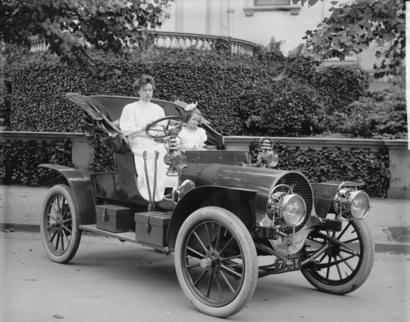
\includegraphics[width=\linewidth]{sample-franklin}
  \caption{1907 Franklin Model D roadster. Photograph by Harris \&
    Ewing, Inc. [Public domain], via Wikimedia
    Commons. (\url{https://goo.gl/VLCRBB}).}
  \Description{A woman and a girl in white dresses sit in an open car.}
\end{figure}

Your figures should contain a caption which describes the figure to
the reader.

Figure captions are placed {\itshape below} the figure.

Every figure should also have a figure description unless it is purely
decorative. These descriptions convey what’s in the image to someone
who cannot see it. They are also used by search engine crawlers for
indexing images, and when images cannot be loaded.

A figure description must be unformatted plain text less than 2000
characters long (including spaces).  {\bfseries Figure descriptions
  should not repeat the figure caption – their purpose is to capture
  important information that is not already provided in the caption or
  the main text of the paper.} For figures that convey important and
complex new information, a short text description may not be
adequate. More complex alternative descriptions can be placed in an
appendix and referenced in a short figure description. For example,
provide a data table capturing the information in a bar chart, or a
structured list representing a graph.  For additional information
regarding how best to write figure descriptions and why doing this is
so important, please see
\url{https://www.acm.org/publications/taps/describing-figures/}.

\subsection{The ``Teaser Figure''}

A ``teaser figure'' is an image, or set of images in one figure, that
are placed after all author and affiliation information, and before
the body of the article, spanning the page. If you wish to have such a
figure in your article, place the command immediately before the
\verb|\maketitle| command:
\begin{verbatim}
  \begin{teaserfigure}
    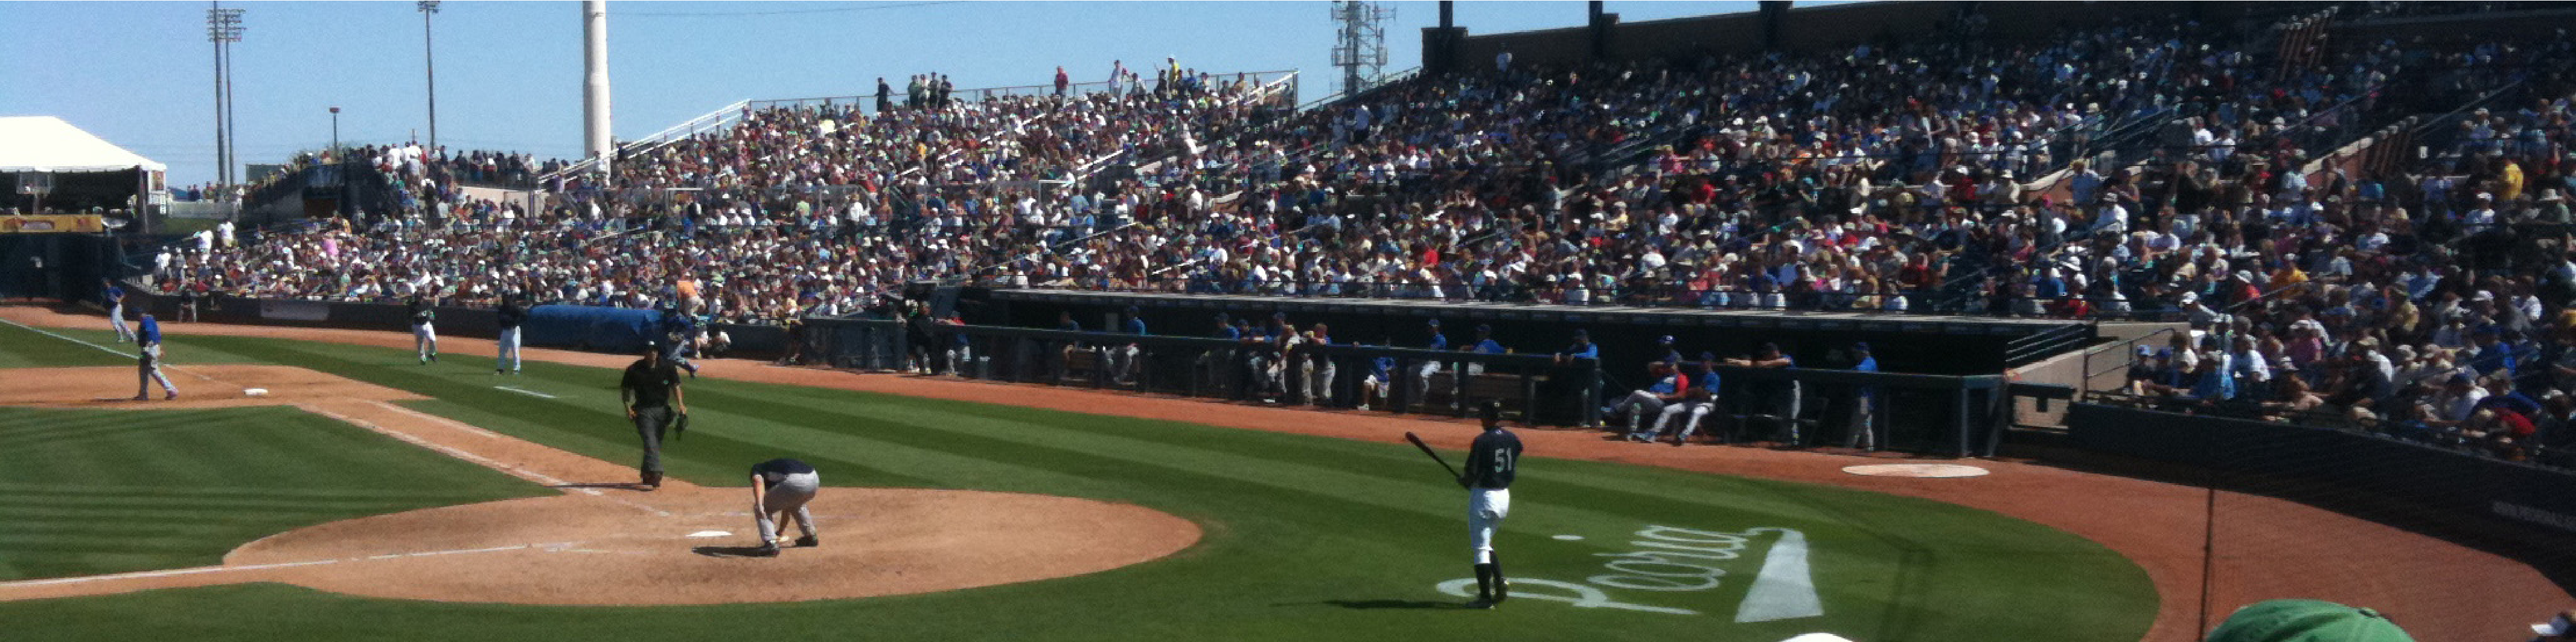
\includegraphics[width=\textwidth]{sampleteaser}
    \caption{figure caption}
    \Description{figure description}
  \end{teaserfigure}
\end{verbatim}

\section{Citations and Bibliographies}

The use of \BibTeX\ for the preparation and formatting of one's
references is strongly recommended. Authors' names should be complete
--- use full first names (``Donald E. Knuth'') not initials
(``D. E. Knuth'') --- and the salient identifying features of a
reference should be included: title, year, volume, number, pages,
article DOI, etc.

The bibliography is included in your source document with these two
commands, placed just before the \verb|\end{document}| command:
\begin{verbatim}
  \bibliographystyle{ACM-Reference-Format}
  \bibliography{bibfile}
\end{verbatim}
where ``\verb|bibfile|'' is the name, without the ``\verb|.bib|''
suffix, of the \BibTeX\ file.

Citations and references are numbered by default. A small number of
ACM publications have citations and references formatted in the
``author year'' style; for these exceptions, please include this
command in the {\bfseries preamble} (before the command
``\verb|\begin{document}|'') of your \LaTeX\ source:
\begin{verbatim}
  \citestyle{acmauthoryear}
\end{verbatim}
Test\citep{de2016trust}...
  Some examples.  A paginated journal article \citep{Abril07}, an
  enumerated journal article \cite{Cohen07}, a reference to an entire
  issue \cite{JCohen96}, a monograph (whole book) \cite{Kosiur01}, a
  monograph/whole book in a series (see 2a in spec. document)
  \cite{Harel79}, a divisible-book such as an anthology or compilation
  \cite{Editor00} followed by the same example, however we only output
  the series if the volume number is given \cite{Editor00a} (so
  Editor00a's series should NOT be present since it has no vol. no.),
  a chapter in a divisible book \cite{Spector90}, a chapter in a
  divisible book in a series \cite{Douglass98}, a multi-volume work as
  book \cite{Knuth97}, a couple of articles in a proceedings (of a
  conference, symposium, workshop for example) (paginated proceedings
  article) \cite{Andler79, Hagerup1993}, a proceedings article with
  all possible elements \cite{Smith10}, an example of an enumerated
  proceedings article \cite{VanGundy07}, an informally published work
  \cite{Harel78}, a couple of preprints \cite{Bornmann2019,
    AnzarootPBM14}, a doctoral dissertation \cite{Clarkson85}, a
  master's thesis: \cite{anisi03}, an online document / world wide web
  resource \cite{Thornburg01, Ablamowicz07, Poker06}, a video game
  (Case 1) \cite{Obama08} and (Case 2) \cite{Novak03} and \cite{Lee05}
  and (Case 3) a patent \cite{JoeScientist001}, work accepted for
  publication \cite{rous08}, 'YYYYb'-test for prolific author
  \cite{SaeediMEJ10} and \cite{SaeediJETC10}. Other cites might
  contain 'duplicate' DOI and URLs (some SIAM articles)
  \cite{Kirschmer:2010:AEI:1958016.1958018}. Boris / Barbara Beeton:
  multi-volume works as books \cite{MR781536} and \cite{MR781537}. A
  couple of citations with DOIs:
  \cite{2004:ITE:1009386.1010128,Kirschmer:2010:AEI:1958016.1958018}. Online
  citations: \cite{TUGInstmem, Thornburg01, CTANacmart}. Artifacts:
  \cite{R} and \cite{UMassCitations}.

\section{Acknowledgments}

Identification of funding sources and other support, and thanks to
individuals and groups that assisted in the research and the
preparation of the work should be included in an acknowledgment
section, which is placed just before the reference section in your
document.

This section has a special environment:
\begin{verbatim}
  \begin{acks}
  ...
  \end{acks}
\end{verbatim}
so that the information contained therein can be more easily collected
during the article metadata extraction phase, and to ensure
consistency in the spelling of the section heading.

Authors should not prepare this section as a numbered or unnumbered {\verb|\section|}; please use the ``{\verb|acks|}'' environment.

\section{Appendices}

If your work needs an appendix, add it before the
``\verb|\end{document}|'' command at the conclusion of your source
document.

Start the appendix with the ``\verb|appendix|'' command:
\begin{verbatim}
  \appendix
\end{verbatim}
and note that in the appendix, sections are lettered, not
numbered. This document has two appendices, demonstrating the section
and subsection identification method.

\section{SIGCHI Extended Abstracts}

The ``\verb|sigchi-a|'' template style (available only in \LaTeX\ and
not in Word) produces a landscape-orientation formatted article, with
a wide left margin. Three environments are available for use with the
``\verb|sigchi-a|'' template style, and produce formatted output in
the margin:
\begin{itemize}
\item {\verb|sidebar|}:  Place formatted text in the margin.
\item {\verb|marginfigure|}: Place a figure in the margin.
\item {\verb|margintable|}: Place a table in the margin.
\end{itemize}

%%
%% The acknowledgments section is defined using the "acks" environment
%% (and NOT an unnumbered section). This ensures the proper
%% identification of the section in the article metadata, and the
%% consistent spelling of the heading.
\begin{acks}
To Robert, for the bagels and explaining CMYK and color spaces.
\end{acks}

%%
%% The next two lines define the bibliography style to be used, and
%% the bibliography file.
%\citestyle{acmauthoryear}
\bibliographystyle{ACM-Reference-Format}

\bibliography{sample-base}

%%
%% If your work has an appendix, this is the place to put it.
\appendix

\section{Research Methods}

\subsection{Part One}

Lorem ipsum dolor sit amet, consectetur adipiscing elit. Morbi
malesuada, quam in pulvinar varius, metus nunc fermentum urna, id
sollicitudin purus odio sit amet enim. Aliquam ullamcorper eu ipsum
vel mollis. Curabitur quis dictum nisl. Phasellus vel semper risus, et
lacinia dolor. Integer ultricies commodo sem nec semper.

\subsection{Part Two}

Etiam commodo feugiat nisl pulvinar pellentesque. Etiam auctor sodales
ligula, non varius nibh pulvinar semper. Suspendisse nec lectus non
ipsum convallis congue hendrerit vitae sapien. Donec at laoreet
eros. Vivamus non purus placerat, scelerisque diam eu, cursus
ante. Etiam aliquam tortor auctor efficitur mattis.

\section{Online Resources}

Nam id fermentum dui. Suspendisse sagittis tortor a nulla mollis, in
pulvinar ex pretium. Sed interdum orci quis metus euismod, et sagittis
enim maximus. Vestibulum gravida massa ut felis suscipit
congue. Quisque mattis elit a risus ultrices commodo venenatis eget
dui. Etiam sagittis eleifend elementum.

Nam interdum magna at lectus dignissim, ac dignissim lorem
rhoncus. Maecenas eu arcu ac neque placerat aliquam. Nunc pulvinar
massa et mattis lacinia.

\end{document}
\endinput
%%
%% End of file `sample-sigconf.tex'.
